
% Default to the notebook output style

    


% Inherit from the specified cell style.




    
\documentclass[11pt]{article}

    
    
    \usepackage[T1]{fontenc}
    % Nicer default font (+ math font) than Computer Modern for most use cases
    \usepackage{mathpazo}

    % Basic figure setup, for now with no caption control since it's done
    % automatically by Pandoc (which extracts ![](path) syntax from Markdown).
    \usepackage{graphicx}
    % We will generate all images so they have a width \maxwidth. This means
    % that they will get their normal width if they fit onto the page, but
    % are scaled down if they would overflow the margins.
    \makeatletter
    \def\maxwidth{\ifdim\Gin@nat@width>\linewidth\linewidth
    \else\Gin@nat@width\fi}
    \makeatother
    \let\Oldincludegraphics\includegraphics
    % Set max figure width to be 80% of text width, for now hardcoded.
    \renewcommand{\includegraphics}[1]{\Oldincludegraphics[width=.8\maxwidth]{#1}}
    % Ensure that by default, figures have no caption (until we provide a
    % proper Figure object with a Caption API and a way to capture that
    % in the conversion process - todo).
    \usepackage{caption}
    \DeclareCaptionLabelFormat{nolabel}{}
    \captionsetup{labelformat=nolabel}

    \usepackage{adjustbox} % Used to constrain images to a maximum size 
    \usepackage{xcolor} % Allow colors to be defined
    \usepackage{enumerate} % Needed for markdown enumerations to work
    \usepackage{geometry} % Used to adjust the document margins
    \usepackage{amsmath} % Equations
    \usepackage{amssymb} % Equations
    \usepackage{textcomp} % defines textquotesingle
    % Hack from http://tex.stackexchange.com/a/47451/13684:
    \AtBeginDocument{%
        \def\PYZsq{\textquotesingle}% Upright quotes in Pygmentized code
    }
    \usepackage{upquote} % Upright quotes for verbatim code
    \usepackage{eurosym} % defines \euro
    \usepackage[mathletters]{ucs} % Extended unicode (utf-8) support
    \usepackage[utf8x]{inputenc} % Allow utf-8 characters in the tex document
    \usepackage{fancyvrb} % verbatim replacement that allows latex
    \usepackage{grffile} % extends the file name processing of package graphics 
                         % to support a larger range 
    % The hyperref package gives us a pdf with properly built
    % internal navigation ('pdf bookmarks' for the table of contents,
    % internal cross-reference links, web links for URLs, etc.)
    \usepackage{hyperref}
    \usepackage{longtable} % longtable support required by pandoc >1.10
    \usepackage{booktabs}  % table support for pandoc > 1.12.2
    \usepackage[inline]{enumitem} % IRkernel/repr support (it uses the enumerate* environment)
    \usepackage[normalem]{ulem} % ulem is needed to support strikethroughs (\sout)
                                % normalem makes italics be italics, not underlines
    

    
    
    % Colors for the hyperref package
    \definecolor{urlcolor}{rgb}{0,.145,.698}
    \definecolor{linkcolor}{rgb}{.71,0.21,0.01}
    \definecolor{citecolor}{rgb}{.12,.54,.11}

    % ANSI colors
    \definecolor{ansi-black}{HTML}{3E424D}
    \definecolor{ansi-black-intense}{HTML}{282C36}
    \definecolor{ansi-red}{HTML}{E75C58}
    \definecolor{ansi-red-intense}{HTML}{B22B31}
    \definecolor{ansi-green}{HTML}{00A250}
    \definecolor{ansi-green-intense}{HTML}{007427}
    \definecolor{ansi-yellow}{HTML}{DDB62B}
    \definecolor{ansi-yellow-intense}{HTML}{B27D12}
    \definecolor{ansi-blue}{HTML}{208FFB}
    \definecolor{ansi-blue-intense}{HTML}{0065CA}
    \definecolor{ansi-magenta}{HTML}{D160C4}
    \definecolor{ansi-magenta-intense}{HTML}{A03196}
    \definecolor{ansi-cyan}{HTML}{60C6C8}
    \definecolor{ansi-cyan-intense}{HTML}{258F8F}
    \definecolor{ansi-white}{HTML}{C5C1B4}
    \definecolor{ansi-white-intense}{HTML}{A1A6B2}

    % commands and environments needed by pandoc snippets
    % extracted from the output of `pandoc -s`
    \providecommand{\tightlist}{%
      \setlength{\itemsep}{0pt}\setlength{\parskip}{0pt}}
    \DefineVerbatimEnvironment{Highlighting}{Verbatim}{commandchars=\\\{\}}
    % Add ',fontsize=\small' for more characters per line
    \newenvironment{Shaded}{}{}
    \newcommand{\KeywordTok}[1]{\textcolor[rgb]{0.00,0.44,0.13}{\textbf{{#1}}}}
    \newcommand{\DataTypeTok}[1]{\textcolor[rgb]{0.56,0.13,0.00}{{#1}}}
    \newcommand{\DecValTok}[1]{\textcolor[rgb]{0.25,0.63,0.44}{{#1}}}
    \newcommand{\BaseNTok}[1]{\textcolor[rgb]{0.25,0.63,0.44}{{#1}}}
    \newcommand{\FloatTok}[1]{\textcolor[rgb]{0.25,0.63,0.44}{{#1}}}
    \newcommand{\CharTok}[1]{\textcolor[rgb]{0.25,0.44,0.63}{{#1}}}
    \newcommand{\StringTok}[1]{\textcolor[rgb]{0.25,0.44,0.63}{{#1}}}
    \newcommand{\CommentTok}[1]{\textcolor[rgb]{0.38,0.63,0.69}{\textit{{#1}}}}
    \newcommand{\OtherTok}[1]{\textcolor[rgb]{0.00,0.44,0.13}{{#1}}}
    \newcommand{\AlertTok}[1]{\textcolor[rgb]{1.00,0.00,0.00}{\textbf{{#1}}}}
    \newcommand{\FunctionTok}[1]{\textcolor[rgb]{0.02,0.16,0.49}{{#1}}}
    \newcommand{\RegionMarkerTok}[1]{{#1}}
    \newcommand{\ErrorTok}[1]{\textcolor[rgb]{1.00,0.00,0.00}{\textbf{{#1}}}}
    \newcommand{\NormalTok}[1]{{#1}}
    
    % Additional commands for more recent versions of Pandoc
    \newcommand{\ConstantTok}[1]{\textcolor[rgb]{0.53,0.00,0.00}{{#1}}}
    \newcommand{\SpecialCharTok}[1]{\textcolor[rgb]{0.25,0.44,0.63}{{#1}}}
    \newcommand{\VerbatimStringTok}[1]{\textcolor[rgb]{0.25,0.44,0.63}{{#1}}}
    \newcommand{\SpecialStringTok}[1]{\textcolor[rgb]{0.73,0.40,0.53}{{#1}}}
    \newcommand{\ImportTok}[1]{{#1}}
    \newcommand{\DocumentationTok}[1]{\textcolor[rgb]{0.73,0.13,0.13}{\textit{{#1}}}}
    \newcommand{\AnnotationTok}[1]{\textcolor[rgb]{0.38,0.63,0.69}{\textbf{\textit{{#1}}}}}
    \newcommand{\CommentVarTok}[1]{\textcolor[rgb]{0.38,0.63,0.69}{\textbf{\textit{{#1}}}}}
    \newcommand{\VariableTok}[1]{\textcolor[rgb]{0.10,0.09,0.49}{{#1}}}
    \newcommand{\ControlFlowTok}[1]{\textcolor[rgb]{0.00,0.44,0.13}{\textbf{{#1}}}}
    \newcommand{\OperatorTok}[1]{\textcolor[rgb]{0.40,0.40,0.40}{{#1}}}
    \newcommand{\BuiltInTok}[1]{{#1}}
    \newcommand{\ExtensionTok}[1]{{#1}}
    \newcommand{\PreprocessorTok}[1]{\textcolor[rgb]{0.74,0.48,0.00}{{#1}}}
    \newcommand{\AttributeTok}[1]{\textcolor[rgb]{0.49,0.56,0.16}{{#1}}}
    \newcommand{\InformationTok}[1]{\textcolor[rgb]{0.38,0.63,0.69}{\textbf{\textit{{#1}}}}}
    \newcommand{\WarningTok}[1]{\textcolor[rgb]{0.38,0.63,0.69}{\textbf{\textit{{#1}}}}}
    
    
    % Define a nice break command that doesn't care if a line doesn't already
    % exist.
    \def\br{\hspace*{\fill} \\* }
    % Math Jax compatability definitions
    \def\gt{>}
    \def\lt{<}
    % Document parameters
    \title{Traffic-Sign-Classifier-WriteUp}
    
    
    

    % Pygments definitions
    
\makeatletter
\def\PY@reset{\let\PY@it=\relax \let\PY@bf=\relax%
    \let\PY@ul=\relax \let\PY@tc=\relax%
    \let\PY@bc=\relax \let\PY@ff=\relax}
\def\PY@tok#1{\csname PY@tok@#1\endcsname}
\def\PY@toks#1+{\ifx\relax#1\empty\else%
    \PY@tok{#1}\expandafter\PY@toks\fi}
\def\PY@do#1{\PY@bc{\PY@tc{\PY@ul{%
    \PY@it{\PY@bf{\PY@ff{#1}}}}}}}
\def\PY#1#2{\PY@reset\PY@toks#1+\relax+\PY@do{#2}}

\expandafter\def\csname PY@tok@ow\endcsname{\let\PY@bf=\textbf\def\PY@tc##1{\textcolor[rgb]{0.67,0.13,1.00}{##1}}}
\expandafter\def\csname PY@tok@si\endcsname{\let\PY@bf=\textbf\def\PY@tc##1{\textcolor[rgb]{0.73,0.40,0.53}{##1}}}
\expandafter\def\csname PY@tok@kd\endcsname{\let\PY@bf=\textbf\def\PY@tc##1{\textcolor[rgb]{0.00,0.50,0.00}{##1}}}
\expandafter\def\csname PY@tok@nb\endcsname{\def\PY@tc##1{\textcolor[rgb]{0.00,0.50,0.00}{##1}}}
\expandafter\def\csname PY@tok@no\endcsname{\def\PY@tc##1{\textcolor[rgb]{0.53,0.00,0.00}{##1}}}
\expandafter\def\csname PY@tok@na\endcsname{\def\PY@tc##1{\textcolor[rgb]{0.49,0.56,0.16}{##1}}}
\expandafter\def\csname PY@tok@c\endcsname{\let\PY@it=\textit\def\PY@tc##1{\textcolor[rgb]{0.25,0.50,0.50}{##1}}}
\expandafter\def\csname PY@tok@sh\endcsname{\def\PY@tc##1{\textcolor[rgb]{0.73,0.13,0.13}{##1}}}
\expandafter\def\csname PY@tok@kc\endcsname{\let\PY@bf=\textbf\def\PY@tc##1{\textcolor[rgb]{0.00,0.50,0.00}{##1}}}
\expandafter\def\csname PY@tok@go\endcsname{\def\PY@tc##1{\textcolor[rgb]{0.53,0.53,0.53}{##1}}}
\expandafter\def\csname PY@tok@gd\endcsname{\def\PY@tc##1{\textcolor[rgb]{0.63,0.00,0.00}{##1}}}
\expandafter\def\csname PY@tok@vc\endcsname{\def\PY@tc##1{\textcolor[rgb]{0.10,0.09,0.49}{##1}}}
\expandafter\def\csname PY@tok@ch\endcsname{\let\PY@it=\textit\def\PY@tc##1{\textcolor[rgb]{0.25,0.50,0.50}{##1}}}
\expandafter\def\csname PY@tok@ss\endcsname{\def\PY@tc##1{\textcolor[rgb]{0.10,0.09,0.49}{##1}}}
\expandafter\def\csname PY@tok@o\endcsname{\def\PY@tc##1{\textcolor[rgb]{0.40,0.40,0.40}{##1}}}
\expandafter\def\csname PY@tok@nv\endcsname{\def\PY@tc##1{\textcolor[rgb]{0.10,0.09,0.49}{##1}}}
\expandafter\def\csname PY@tok@nc\endcsname{\let\PY@bf=\textbf\def\PY@tc##1{\textcolor[rgb]{0.00,0.00,1.00}{##1}}}
\expandafter\def\csname PY@tok@s1\endcsname{\def\PY@tc##1{\textcolor[rgb]{0.73,0.13,0.13}{##1}}}
\expandafter\def\csname PY@tok@il\endcsname{\def\PY@tc##1{\textcolor[rgb]{0.40,0.40,0.40}{##1}}}
\expandafter\def\csname PY@tok@mi\endcsname{\def\PY@tc##1{\textcolor[rgb]{0.40,0.40,0.40}{##1}}}
\expandafter\def\csname PY@tok@c1\endcsname{\let\PY@it=\textit\def\PY@tc##1{\textcolor[rgb]{0.25,0.50,0.50}{##1}}}
\expandafter\def\csname PY@tok@fm\endcsname{\def\PY@tc##1{\textcolor[rgb]{0.00,0.00,1.00}{##1}}}
\expandafter\def\csname PY@tok@vi\endcsname{\def\PY@tc##1{\textcolor[rgb]{0.10,0.09,0.49}{##1}}}
\expandafter\def\csname PY@tok@w\endcsname{\def\PY@tc##1{\textcolor[rgb]{0.73,0.73,0.73}{##1}}}
\expandafter\def\csname PY@tok@mb\endcsname{\def\PY@tc##1{\textcolor[rgb]{0.40,0.40,0.40}{##1}}}
\expandafter\def\csname PY@tok@gp\endcsname{\let\PY@bf=\textbf\def\PY@tc##1{\textcolor[rgb]{0.00,0.00,0.50}{##1}}}
\expandafter\def\csname PY@tok@err\endcsname{\def\PY@bc##1{\setlength{\fboxsep}{0pt}\fcolorbox[rgb]{1.00,0.00,0.00}{1,1,1}{\strut ##1}}}
\expandafter\def\csname PY@tok@sa\endcsname{\def\PY@tc##1{\textcolor[rgb]{0.73,0.13,0.13}{##1}}}
\expandafter\def\csname PY@tok@k\endcsname{\let\PY@bf=\textbf\def\PY@tc##1{\textcolor[rgb]{0.00,0.50,0.00}{##1}}}
\expandafter\def\csname PY@tok@kp\endcsname{\def\PY@tc##1{\textcolor[rgb]{0.00,0.50,0.00}{##1}}}
\expandafter\def\csname PY@tok@sx\endcsname{\def\PY@tc##1{\textcolor[rgb]{0.00,0.50,0.00}{##1}}}
\expandafter\def\csname PY@tok@nl\endcsname{\def\PY@tc##1{\textcolor[rgb]{0.63,0.63,0.00}{##1}}}
\expandafter\def\csname PY@tok@ge\endcsname{\let\PY@it=\textit}
\expandafter\def\csname PY@tok@sc\endcsname{\def\PY@tc##1{\textcolor[rgb]{0.73,0.13,0.13}{##1}}}
\expandafter\def\csname PY@tok@dl\endcsname{\def\PY@tc##1{\textcolor[rgb]{0.73,0.13,0.13}{##1}}}
\expandafter\def\csname PY@tok@s\endcsname{\def\PY@tc##1{\textcolor[rgb]{0.73,0.13,0.13}{##1}}}
\expandafter\def\csname PY@tok@bp\endcsname{\def\PY@tc##1{\textcolor[rgb]{0.00,0.50,0.00}{##1}}}
\expandafter\def\csname PY@tok@vm\endcsname{\def\PY@tc##1{\textcolor[rgb]{0.10,0.09,0.49}{##1}}}
\expandafter\def\csname PY@tok@nt\endcsname{\let\PY@bf=\textbf\def\PY@tc##1{\textcolor[rgb]{0.00,0.50,0.00}{##1}}}
\expandafter\def\csname PY@tok@kt\endcsname{\def\PY@tc##1{\textcolor[rgb]{0.69,0.00,0.25}{##1}}}
\expandafter\def\csname PY@tok@cs\endcsname{\let\PY@it=\textit\def\PY@tc##1{\textcolor[rgb]{0.25,0.50,0.50}{##1}}}
\expandafter\def\csname PY@tok@ni\endcsname{\let\PY@bf=\textbf\def\PY@tc##1{\textcolor[rgb]{0.60,0.60,0.60}{##1}}}
\expandafter\def\csname PY@tok@nd\endcsname{\def\PY@tc##1{\textcolor[rgb]{0.67,0.13,1.00}{##1}}}
\expandafter\def\csname PY@tok@gh\endcsname{\let\PY@bf=\textbf\def\PY@tc##1{\textcolor[rgb]{0.00,0.00,0.50}{##1}}}
\expandafter\def\csname PY@tok@cm\endcsname{\let\PY@it=\textit\def\PY@tc##1{\textcolor[rgb]{0.25,0.50,0.50}{##1}}}
\expandafter\def\csname PY@tok@gr\endcsname{\def\PY@tc##1{\textcolor[rgb]{1.00,0.00,0.00}{##1}}}
\expandafter\def\csname PY@tok@cpf\endcsname{\let\PY@it=\textit\def\PY@tc##1{\textcolor[rgb]{0.25,0.50,0.50}{##1}}}
\expandafter\def\csname PY@tok@s2\endcsname{\def\PY@tc##1{\textcolor[rgb]{0.73,0.13,0.13}{##1}}}
\expandafter\def\csname PY@tok@ne\endcsname{\let\PY@bf=\textbf\def\PY@tc##1{\textcolor[rgb]{0.82,0.25,0.23}{##1}}}
\expandafter\def\csname PY@tok@nf\endcsname{\def\PY@tc##1{\textcolor[rgb]{0.00,0.00,1.00}{##1}}}
\expandafter\def\csname PY@tok@kr\endcsname{\let\PY@bf=\textbf\def\PY@tc##1{\textcolor[rgb]{0.00,0.50,0.00}{##1}}}
\expandafter\def\csname PY@tok@se\endcsname{\let\PY@bf=\textbf\def\PY@tc##1{\textcolor[rgb]{0.73,0.40,0.13}{##1}}}
\expandafter\def\csname PY@tok@cp\endcsname{\def\PY@tc##1{\textcolor[rgb]{0.74,0.48,0.00}{##1}}}
\expandafter\def\csname PY@tok@nn\endcsname{\let\PY@bf=\textbf\def\PY@tc##1{\textcolor[rgb]{0.00,0.00,1.00}{##1}}}
\expandafter\def\csname PY@tok@mo\endcsname{\def\PY@tc##1{\textcolor[rgb]{0.40,0.40,0.40}{##1}}}
\expandafter\def\csname PY@tok@gs\endcsname{\let\PY@bf=\textbf}
\expandafter\def\csname PY@tok@mf\endcsname{\def\PY@tc##1{\textcolor[rgb]{0.40,0.40,0.40}{##1}}}
\expandafter\def\csname PY@tok@mh\endcsname{\def\PY@tc##1{\textcolor[rgb]{0.40,0.40,0.40}{##1}}}
\expandafter\def\csname PY@tok@vg\endcsname{\def\PY@tc##1{\textcolor[rgb]{0.10,0.09,0.49}{##1}}}
\expandafter\def\csname PY@tok@gi\endcsname{\def\PY@tc##1{\textcolor[rgb]{0.00,0.63,0.00}{##1}}}
\expandafter\def\csname PY@tok@sr\endcsname{\def\PY@tc##1{\textcolor[rgb]{0.73,0.40,0.53}{##1}}}
\expandafter\def\csname PY@tok@sb\endcsname{\def\PY@tc##1{\textcolor[rgb]{0.73,0.13,0.13}{##1}}}
\expandafter\def\csname PY@tok@kn\endcsname{\let\PY@bf=\textbf\def\PY@tc##1{\textcolor[rgb]{0.00,0.50,0.00}{##1}}}
\expandafter\def\csname PY@tok@sd\endcsname{\let\PY@it=\textit\def\PY@tc##1{\textcolor[rgb]{0.73,0.13,0.13}{##1}}}
\expandafter\def\csname PY@tok@m\endcsname{\def\PY@tc##1{\textcolor[rgb]{0.40,0.40,0.40}{##1}}}
\expandafter\def\csname PY@tok@gu\endcsname{\let\PY@bf=\textbf\def\PY@tc##1{\textcolor[rgb]{0.50,0.00,0.50}{##1}}}
\expandafter\def\csname PY@tok@gt\endcsname{\def\PY@tc##1{\textcolor[rgb]{0.00,0.27,0.87}{##1}}}

\def\PYZbs{\char`\\}
\def\PYZus{\char`\_}
\def\PYZob{\char`\{}
\def\PYZcb{\char`\}}
\def\PYZca{\char`\^}
\def\PYZam{\char`\&}
\def\PYZlt{\char`\<}
\def\PYZgt{\char`\>}
\def\PYZsh{\char`\#}
\def\PYZpc{\char`\%}
\def\PYZdl{\char`\$}
\def\PYZhy{\char`\-}
\def\PYZsq{\char`\'}
\def\PYZdq{\char`\"}
\def\PYZti{\char`\~}
% for compatibility with earlier versions
\def\PYZat{@}
\def\PYZlb{[}
\def\PYZrb{]}
\makeatother


    % Exact colors from NB
    \definecolor{incolor}{rgb}{0.0, 0.0, 0.5}
    \definecolor{outcolor}{rgb}{0.545, 0.0, 0.0}



    
    % Prevent overflowing lines due to hard-to-break entities
    \sloppy 
    % Setup hyperref package
    \hypersetup{
      breaklinks=true,  % so long urls are correctly broken across lines
      colorlinks=true,
      urlcolor=urlcolor,
      linkcolor=linkcolor,
      citecolor=citecolor,
      }
    % Slightly bigger margins than the latex defaults
    
    \geometry{verbose,tmargin=1in,bmargin=1in,lmargin=1in,rmargin=1in}
    
    

    \begin{document}
    
    
    \maketitle
    
    

    
    \hypertarget{traffic-sign-recognition}{%
\section{\texorpdfstring{\textbf{Traffic Sign
Recognition}}{Traffic Sign Recognition}}\label{traffic-sign-recognition}}

\hypertarget{writeup}{%
\subsection{Writeup}\label{writeup}}

\hypertarget{you-can-use-this-file-as-a-template-for-your-writeup-if-you-want-to-submit-it-as-a-markdown-file-but-feel-free-to-use-some-other-method-and-submit-a-pdf-if-you-prefer.}{%
\subsubsection{You can use this file as a template for your writeup if
you want to submit it as a markdown file, but feel free to use some
other method and submit a pdf if you
prefer.}\label{you-can-use-this-file-as-a-template-for-your-writeup-if-you-want-to-submit-it-as-a-markdown-file-but-feel-free-to-use-some-other-method-and-submit-a-pdf-if-you-prefer.}}

\begin{center}\rule{0.5\linewidth}{\linethickness}\end{center}

\textbf{Build a Traffic Sign Recognition Project}

The goals / steps of this project are the following: * Load the data set
(see below for links to the project data set) * Explore, summarize and
visualize the data set * Design, train and test a model architecture *
Use the model to make predictions on new images * Analyze the softmax
probabilities of the new images * Summarize the results with a written
report

\hypertarget{rubric-points}{%
\subsection{Rubric Points}\label{rubric-points}}

\hypertarget{here-i-will-consider-the-rubric-points-individually-and-describe-how-i-addressed-each-point-in-my-implementation.}{%
\subsubsection{\texorpdfstring{Here I will consider the
\href{https://review.udacity.com/\#!/rubrics/481/view}{rubric points}
individually and describe how I addressed each point in my
implementation.}{Here I will consider the rubric points individually and describe how I addressed each point in my implementation.}}\label{here-i-will-consider-the-rubric-points-individually-and-describe-how-i-addressed-each-point-in-my-implementation.}}

\begin{center}\rule{0.5\linewidth}{\linethickness}\end{center}

\hypertarget{writeup-readme}{%
\subsubsection{Writeup / README}\label{writeup-readme}}

\hypertarget{provide-a-writeup-readme-that-includes-all-the-rubric-points-and-how-you-addressed-each-one.-you-can-submit-your-writeup-as-markdown-or-pdf.-you-can-use-this-template-as-a-guide-for-writing-the-report.-the-submission-includes-the-project-code.}{%
\paragraph{1. Provide a Writeup / README that includes all the rubric
points and how you addressed each one. You can submit your writeup as
markdown or pdf. You can use this template as a guide for writing the
report. The submission includes the project
code.}\label{provide-a-writeup-readme-that-includes-all-the-rubric-points-and-how-you-addressed-each-one.-you-can-submit-your-writeup-as-markdown-or-pdf.-you-can-use-this-template-as-a-guide-for-writing-the-report.-the-submission-includes-the-project-code.}}

You're reading it!

\hypertarget{data-set-summary-exploration}{%
\subsubsection{Data Set Summary \&
Exploration}\label{data-set-summary-exploration}}

\hypertarget{provide-a-basic-summary-of-the-data-set.-in-the-code-the-analysis-should-be-done-using-python-numpy-andor-pandas-methods-rather-than-hardcoding-results-manually.}{%
\paragraph{1. Provide a basic summary of the data set. In the code, the
analysis should be done using python, numpy and/or pandas methods rather
than hardcoding results
manually.}\label{provide-a-basic-summary-of-the-data-set.-in-the-code-the-analysis-should-be-done-using-python-numpy-andor-pandas-methods-rather-than-hardcoding-results-manually.}}

I used the pandas library to calculate summary statistics of the traffic
signs data set:

\begin{itemize}
\tightlist
\item
  The size of training set is 34799
\item
  The size of the validation set is 4410
\item
  The size of test set is 12630
\item
  The shape of a traffic sign image is 32 x 32 x 3 (RGB)
\item
  The number of unique classes/labels in the data set is 43
\end{itemize}

See code in Step 1 (\textbf{Traffic\_Sign\_ClassifierFinal.ipynb}).

\hypertarget{include-an-exploratory-visualization-of-the-dataset.}{%
\paragraph{2. Include an exploratory visualization of the
dataset.}\label{include-an-exploratory-visualization-of-the-dataset.}}

The below are exploratory visualizations of the dataset.

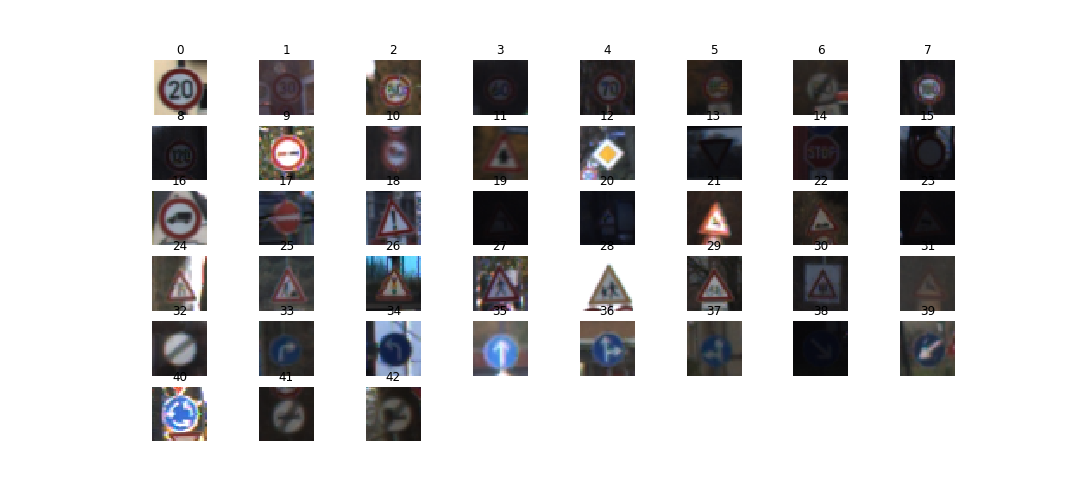
\includegraphics{./images/classes_vis.png}
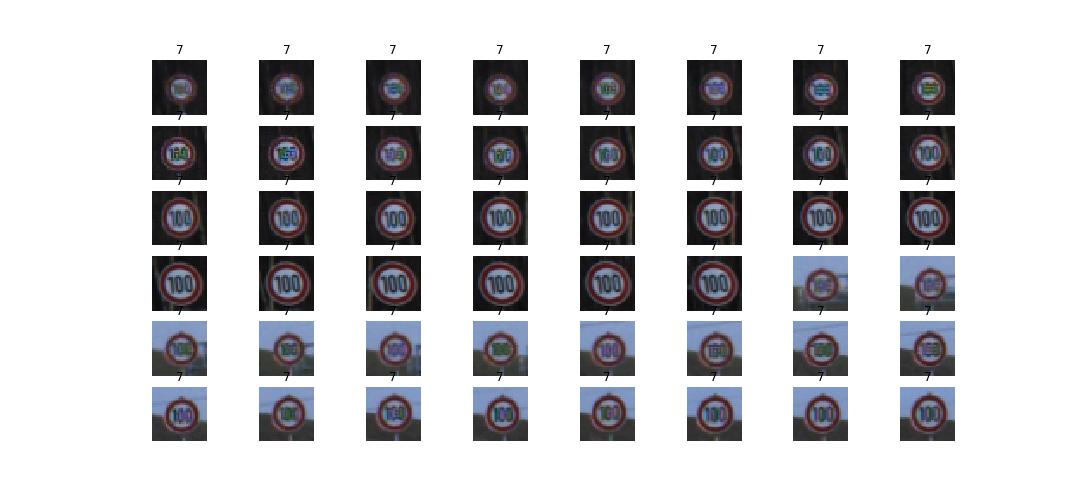
\includegraphics{./images/class_vis.png}

\begin{itemize}
\item
  Many images have different perspective, sign size, brightness and
  background. This is especially visible in the images for a particular
  class (here it is the 100 km/h speed limit).
\item
  All the images are in the same size of 32 x 32 px (RGB).
\item
  The next bar charts illustrate a distribution of images across
  datasets. It is clear from the histograms that some classes are
  underrepresented. This might results in a lower performance of the ANN
  for these signs. Following the recommendation from
  \href{http://yann.lecun.com/exdb/publis/pdf/sermanet-ijcnn-11.pdf}{Traffic
  Sign Recognition with Multi-Scale Convolutional Networks}, a fake
  images (jittered) should be added to a dataset.
  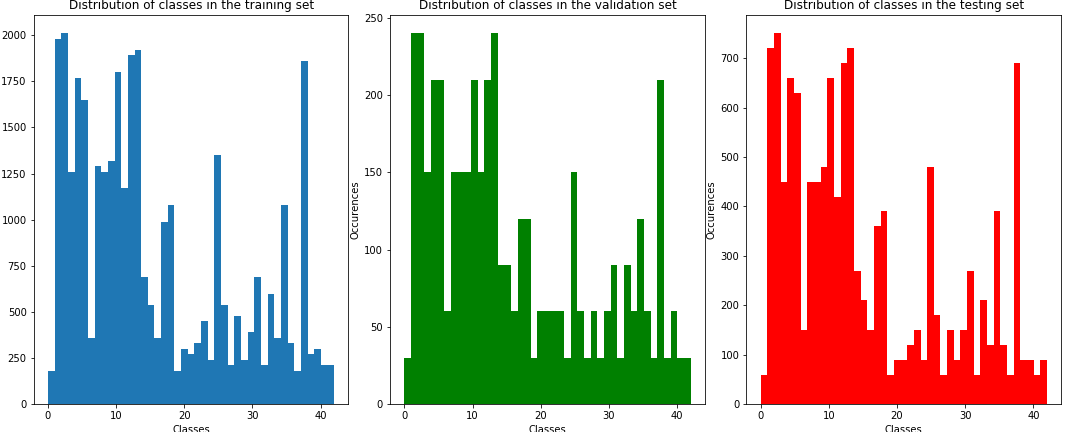
\includegraphics{./images/dataset_dist.png}
\end{itemize}

See code in Step 1 (\textbf{Traffic\_Sign\_ClassifierFinal.ipynb}).

\hypertarget{design-and-test-a-model-architecture}{%
\subsubsection{Design and Test a Model
Architecture}\label{design-and-test-a-model-architecture}}

\hypertarget{describe-how-you-preprocessed-the-image-data.-what-techniques-were-chosen-and-why-did-you-choose-these-techniques-consider-including-images-showing-the-output-of-each-preprocessing-technique.-pre-processing-refers-to-techniques-such-as-converting-to-grayscale-normalization-etc.-optional-as-described-in-the-stand-out-suggestions-part-of-the-rubric-if-you-generated-additional-data-for-training-describe-why-you-decided-to-generate-additional-data-how-you-generated-the-data-and-provide-example-images-of-the-additional-data.-then-describe-the-characteristics-of-the-augmented-training-set-like-number-of-images-in-the-set-number-of-images-for-each-class-etc.}{%
\paragraph{1. Describe how you preprocessed the image data. What
techniques were chosen and why did you choose these techniques? Consider
including images showing the output of each preprocessing technique.
Pre-processing refers to techniques such as converting to grayscale,
normalization, etc. (OPTIONAL: As described in the ``Stand Out
Suggestions'' part of the rubric, if you generated additional data for
training, describe why you decided to generate additional data, how you
generated the data, and provide example images of the additional data.
Then describe the characteristics of the augmented training set like
number of images in the set, number of images for each class,
etc.)}\label{describe-how-you-preprocessed-the-image-data.-what-techniques-were-chosen-and-why-did-you-choose-these-techniques-consider-including-images-showing-the-output-of-each-preprocessing-technique.-pre-processing-refers-to-techniques-such-as-converting-to-grayscale-normalization-etc.-optional-as-described-in-the-stand-out-suggestions-part-of-the-rubric-if-you-generated-additional-data-for-training-describe-why-you-decided-to-generate-additional-data-how-you-generated-the-data-and-provide-example-images-of-the-additional-data.-then-describe-the-characteristics-of-the-augmented-training-set-like-number-of-images-in-the-set-number-of-images-for-each-class-etc.}}

The most of improvements were inspired from the
\href{http://yann.lecun.com/exdb/publis/pdf/sermanet-ijcnn-11.pdf}{Traffic
Sign Recognition with Multi-Scale Convolutional Networks} and from a
classroom exercise with the LeNet implementation.

\begin{itemize}
\item
  Conversion to grayscale - Not much improvement recorded. However, it
  seems that training time is shorter than for a 3-channels image. This
  can be useful if large datasets are used e.g.~when jittered images are
  added.
\item
  Standardisation to between -1 and 1 - Easy to implement and worked
  very well. However, it is important to have a result as float,
  otherwise the effect is quite opposite; a bid drop in the accuracy.
\item
  Conversion to YUV and normalisation of Y channel - A noticeable
  improvement with respect to initial 89\% but in the later stage of the
  project this technique was dismissed in favour of the global
  normalisation and standardisation.
\item
  Global normalisation - Implemented with use of cv2.equalizeHist().
  This provided a significant boost to the training and validation
  accuracy. Very likely the increased contrast (see figure below) helps
  the network to extract more features.
  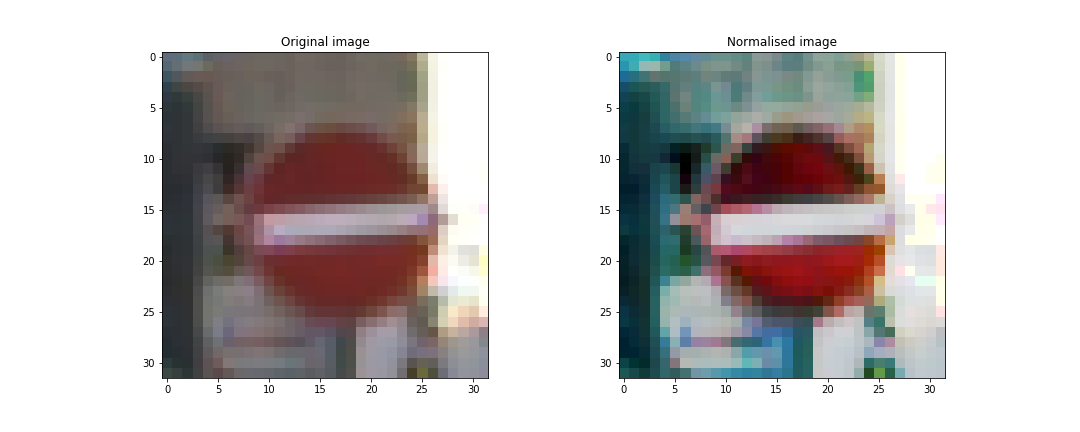
\includegraphics{./images/normalised.png}
\item
  Additional data - The histograms of the original dataset indicated
  that the classes were not equally represented by the number of images.
  Also, the mentioned article suggested to add few additional augmented
  images per each original image. The suggested augmentations were:
  random translation by {[}-2:2{]} pixels, random rotation within
  {[}-15: +15{]} degrees and random scaling within {[}-10:10{]} \%. Here
  is an example of an original image and an augmented image:
  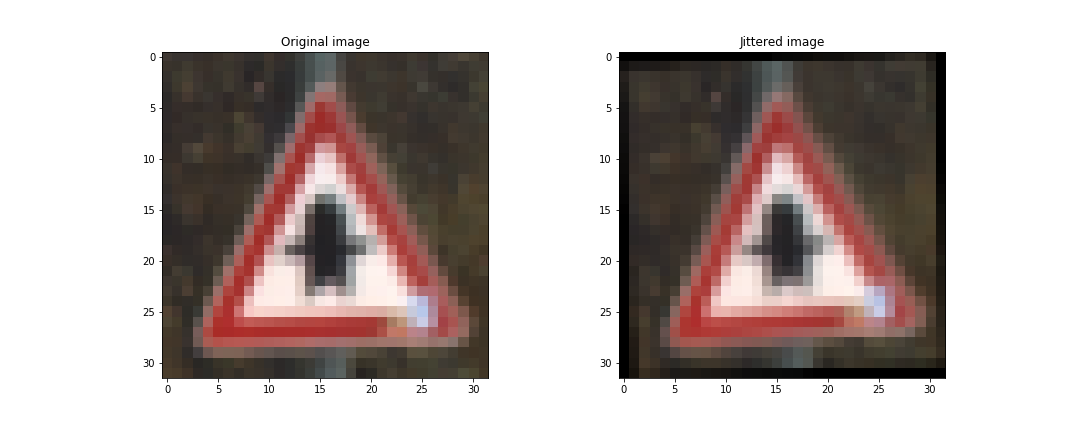
\includegraphics{./images/jittered.png}
\item
  The original dataset has 34799 images whereas the augmented dataset
  contains 208794 images. The augmentation introduced another
  significant boost, allowing to consistently achieving the validation
  accuracy above 96\%.
\end{itemize}

Final pre-processing involves: Step 1: Global normalisation Step 2:
Standardisation Step 3: Generate additional jittered images

See code in Step 2:Pre-process the Data Set
(\textbf{Traffic\_Sign\_ClassifierFinal.ipynb}).

\hypertarget{describe-what-your-final-model-architecture-looks-like-including-model-type-layers-layer-sizes-connectivity-etc.-consider-including-a-diagram-andor-table-describing-the-final-model.}{%
\paragraph{2. Describe what your final model architecture looks like
including model type, layers, layer sizes, connectivity, etc.) Consider
including a diagram and/or table describing the final
model.}\label{describe-what-your-final-model-architecture-looks-like-including-model-type-layers-layer-sizes-connectivity-etc.-consider-including-a-diagram-andor-table-describing-the-final-model.}}

The LeNet network, as suggested, was chosen as a base for my model. The
mentioned paper suggested further modifications but once a dropout was
added after each layer the model started to perform very well and focus
was placed on tuning the hyperparameters and adding fake data.

My final model consisted of the following layers:

\begin{longtable}[]{@{}cc@{}}
\toprule
Layer & Description\tabularnewline
\midrule
\endhead
Input & 32x32x3 RGB image\tabularnewline
Convolution 5x5 & 1x1 stride, valid padding, outputs
28x28x12\tabularnewline
RELU &\tabularnewline
Dropout & 0.9\tabularnewline
Max pooling & 2x2 stride, same padding, outputs 14x14x6\tabularnewline
Dropout & 0.9\tabularnewline
Convolution 5x5 & 1x1 stride, valid padding, outputs
10x10x16\tabularnewline
RELU &\tabularnewline
Dropout & 0.9\tabularnewline
Max pooling & 2x2 stride, same padding, outputs 5x5x16\tabularnewline
Dropout & 0.9\tabularnewline
Flatten & outputs 400\tabularnewline
Fully connected & outputs 120\tabularnewline
RELU &\tabularnewline
Dropout & 0.9\tabularnewline
Fully connected & outputs 84\tabularnewline
RELU &\tabularnewline
Dropout & 0.9\tabularnewline
Fully connected & outputs 43\tabularnewline
\bottomrule
\end{longtable}

See code in Step 2: Architecture
(\textbf{Traffic\_Sign\_ClassifierFinal.ipynb}).

\hypertarget{describe-how-you-trained-your-model.-the-discussion-can-include-the-type-of-optimizer-the-batch-size-number-of-epochs-and-any-hyperparameters-such-as-learning-rate.}{%
\paragraph{3. Describe how you trained your model. The discussion can
include the type of optimizer, the batch size, number of epochs and any
hyperparameters such as learning
rate.}\label{describe-how-you-trained-your-model.-the-discussion-can-include-the-type-of-optimizer-the-batch-size-number-of-epochs-and-any-hyperparameters-such-as-learning-rate.}}

\begin{itemize}
\tightlist
\item
  The Adam Optimiser as a default optimiser performed very well. The
  Gradient Descent Optimizer was also tried few times but its
  performance was worse than Adam's.
\item
  The hyperparameters were adjust by trial and error. The final settings
  were Epochs=30, Batch=128, learning rate=0.0005, dropout probability
  0.9 (10\%), mu=0, sigma=0.1,
\item
  Training time was quite fast and took approximately just several
  minutes on the NVIDA GTX 980. However, making TensorFlow to work on a
  GPU required quite some time.
\end{itemize}

See code in Step 2:Train, Validate and Test the Model
(\textbf{Traffic\_Sign\_ClassifierFinal.ipynb}).

\hypertarget{describe-the-approach-taken-for-finding-a-solution-and-getting-the-validation-set-accuracy-to-be-at-least-0.93.-include-in-the-discussion-the-results-on-the-training-validation-and-test-sets-and-where-in-the-code-these-were-calculated.-your-approach-may-have-been-an-iterative-process-in-which-case-outline-the-steps-you-took-to-get-to-the-final-solution-and-why-you-chose-those-steps.-perhaps-your-solution-involved-an-already-well-known-implementation-or-architecture.-in-this-case-discuss-why-you-think-the-architecture-is-suitable-for-the-current-problem.}{%
\paragraph{4. Describe the approach taken for finding a solution and
getting the validation set accuracy to be at least 0.93. Include in the
discussion the results on the training, validation and test sets and
where in the code these were calculated. Your approach may have been an
iterative process, in which case, outline the steps you took to get to
the final solution and why you chose those steps. Perhaps your solution
involved an already well known implementation or architecture. In this
case, discuss why you think the architecture is suitable for the current
problem.}\label{describe-the-approach-taken-for-finding-a-solution-and-getting-the-validation-set-accuracy-to-be-at-least-0.93.-include-in-the-discussion-the-results-on-the-training-validation-and-test-sets-and-where-in-the-code-these-were-calculated.-your-approach-may-have-been-an-iterative-process-in-which-case-outline-the-steps-you-took-to-get-to-the-final-solution-and-why-you-chose-those-steps.-perhaps-your-solution-involved-an-already-well-known-implementation-or-architecture.-in-this-case-discuss-why-you-think-the-architecture-is-suitable-for-the-current-problem.}}

My final model results were: * training set accuracy of 100\% *
validation set accuracy of 98.5\% * test set accuracy of 96.6\%

If an iterative approach was chosen: * What was the first architecture
that was tried and why was it chosen? The adopted LeNet network from the
classroom's handwriting exercise produced good initial results i.e.~89\%
hence it was used. * What were some problems with the initial
architecture? A correct adoption in terms of layers sizes and selection
of a correct sigma parameter. Once sigma was changed from 0.01 to 0.1
much better results were obtained. * How was the architecture adjusted
and why was it adjusted? Typical adjustments could include choosing a
different model architecture, adding or taking away layers (pooling,
dropout, convolution, etc), using an activation function or changing the
activation function. One common justification for adjusting an
architecture would be due to overfitting or underfitting. A high
accuracy on the training set but low accuracy on the validation set
indicates over fitting; a low accuracy on both sets indicates under
fitting. The attempt to replicate the suggested architecture as in the
\href{http://yann.lecun.com/exdb/publis/pdf/sermanet-ijcnn-11.pdf}{Traffic
Sign Recognition with Multi-Scale Convolutional Networks} failed.
Instead a dropout of 10\% was introduced after each layer to address the
overfitting. Different level of dropout was tried but 10\% seem to work
the best for my model. * Which parameters were tuned? How were they
adjusted and why? The batch size and epochs were set fixed for most of
trials. The major tuning parameter was the learning rate. It was
initially set to 0.001 but gradually it was reduced to 0.0008 and then
to 0.0005. * What are some of the important design choices and why were
they chosen? For example, why might a convolution layer work well with
this problem? How might a dropout layer help with creating a successful
model? It was noticed that the model was overfitting. To address this a
dropout was added. The introduction of dropout was one of the major
boosts to the model's accuracy.

If a well known architecture was chosen: * What architecture was chosen?
* Why did you believe it would be relevant to the traffic sign
application? The convolutional networks used in the LeNet network and
the mentioned paper demonstrated very good performance in symbols
recognition. And as stated in the paper they can work in real time on
embedded systems makes them an excellent tool for autonomous vehicles. *
How does the final model's accuracy on the training, validation and test
set provide evidence that the model is working well? 96.6\% out of 12630
images were predicted correctly which is strong enough evidence that
model works well. However, 4410 images for a validation set seem to be
not enough to accurately monitor training progres. Further work would
increase this amount to approx. 20\% of a training dataset size.

\hypertarget{test-a-model-on-new-images}{%
\subsubsection{Test a Model on New
Images}\label{test-a-model-on-new-images}}

\hypertarget{choose-five-german-traffic-signs-found-on-the-web-and-provide-them-in-the-report.-for-each-image-discuss-what-quality-or-qualities-might-be-difficult-to-classify.}{%
\paragraph{1. Choose five German traffic signs found on the web and
provide them in the report. For each image, discuss what quality or
qualities might be difficult to
classify.}\label{choose-five-german-traffic-signs-found-on-the-web-and-provide-them-in-the-report.-for-each-image-discuss-what-quality-or-qualities-might-be-difficult-to-classify.}}

Here are 9 German traffic signs that I found on the web:

\begin{figure}
\centering

\includegraphics{./images/testsigns.png}
\caption{alt text}
\end{figure}

The images are different in quality and size; they were cropped out from
the original images.

The yield, no vehicles and no entry signs should be easy to recognise
due to their unique features. Next 4 signs are triangular with a red
border and black symbol. It expected these would be a bigger challenge
for a model. The final two sings for speed limits also share some
similar features so it would be interesting to see if the model can
distinguish them correctly.

The images were resized into 32x32 RGB px with use of cv2.resize(, ,
interpolation=cv2.INTER\_AREA). The interpolation can play significant
role so it was chosen such way the imported images resemble the quality
of images from the training set.

See code in Step 3: Load and Output the Images
(\textbf{Traffic\_Sign\_ClassifierFinal.ipynb}).

\hypertarget{discuss-the-models-predictions-on-these-new-traffic-signs-and-compare-the-results-to-predicting-on-the-test-set.-at-a-minimum-discuss-what-the-predictions-were-the-accuracy-on-these-new-predictions-and-compare-the-accuracy-to-the-accuracy-on-the-test-set-optional-discuss-the-results-in-more-detail-as-described-in-the-stand-out-suggestions-part-of-the-rubric.}{%
\paragraph{2. Discuss the model's predictions on these new traffic signs
and compare the results to predicting on the test set. At a minimum,
discuss what the predictions were, the accuracy on these new
predictions, and compare the accuracy to the accuracy on the test set
(OPTIONAL: Discuss the results in more detail as described in the
``Stand Out Suggestions'' part of the
rubric).}\label{discuss-the-models-predictions-on-these-new-traffic-signs-and-compare-the-results-to-predicting-on-the-test-set.-at-a-minimum-discuss-what-the-predictions-were-the-accuracy-on-these-new-predictions-and-compare-the-accuracy-to-the-accuracy-on-the-test-set-optional-discuss-the-results-in-more-detail-as-described-in-the-stand-out-suggestions-part-of-the-rubric.}}

Here are the results of the prediction:
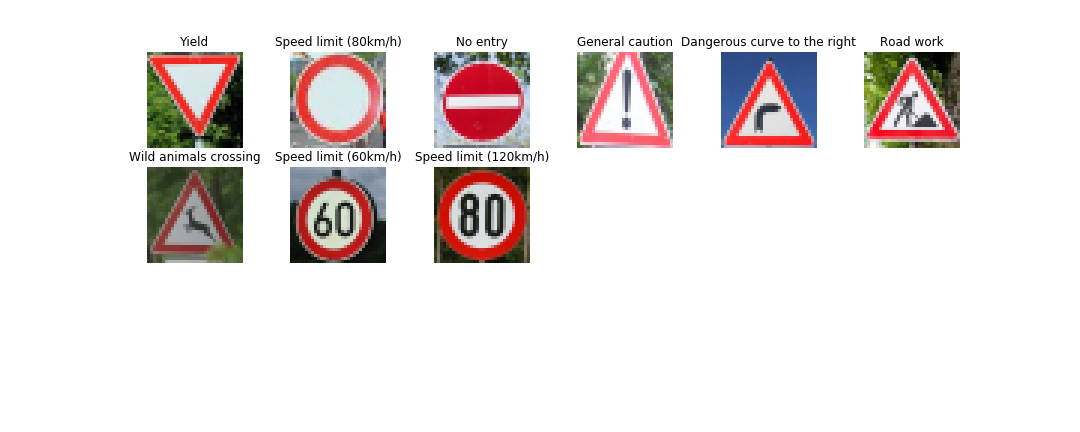
\includegraphics{./images/predictions.png}

\begin{longtable}[]{@{}cc@{}}
\toprule
Image & Prediction\tabularnewline
\midrule
\endhead
Yield & Yield\tabularnewline
No vehicles & \textbf{Speed limit 80km/h}\tabularnewline
No entry & No entry\tabularnewline
General caution & General caution\tabularnewline
Dangerous curve to the right & Dangerous curve to the
right\tabularnewline
Road work & Road work\tabularnewline
Wild animals & Wild animals\tabularnewline
Speed limit 60km/h & Speed limit 60km/h\tabularnewline
Speed limit 80km/h & \textbf{Speed limit 120km/h}\tabularnewline
\bottomrule
\end{longtable}

The model was able to correctly guess 7 of the 9 traffic signs, which
gives an accuracy of 77.78\%.

See code in Step 3: Predict the Sign Type for Each Image
(\textbf{Traffic\_Sign\_ClassifierFinal.ipynb}).

\hypertarget{describe-how-certain-the-model-is-when-predicting-on-each-of-the-five-new-images-by-looking-at-the-softmax-probabilities-for-each-prediction.-provide-the-top-5-softmax-probabilities-for-each-image-along-with-the-sign-type-of-each-probability.-optional-as-described-in-the-stand-out-suggestions-part-of-the-rubric-visualizations-can-also-be-provided-such-as-bar-charts}{%
\paragraph{3. Describe how certain the model is when predicting on each
of the five new images by looking at the softmax probabilities for each
prediction. Provide the top 5 softmax probabilities for each image along
with the sign type of each probability. (OPTIONAL: as described in the
``Stand Out Suggestions'' part of the rubric, visualizations can also be
provided such as bar
charts)}\label{describe-how-certain-the-model-is-when-predicting-on-each-of-the-five-new-images-by-looking-at-the-softmax-probabilities-for-each-prediction.-provide-the-top-5-softmax-probabilities-for-each-image-along-with-the-sign-type-of-each-probability.-optional-as-described-in-the-stand-out-suggestions-part-of-the-rubric-visualizations-can-also-be-provided-such-as-bar-charts}}

The bar charts below visualise the softmax probabilities for each image
found on the web.

\begin{figure}
\centering
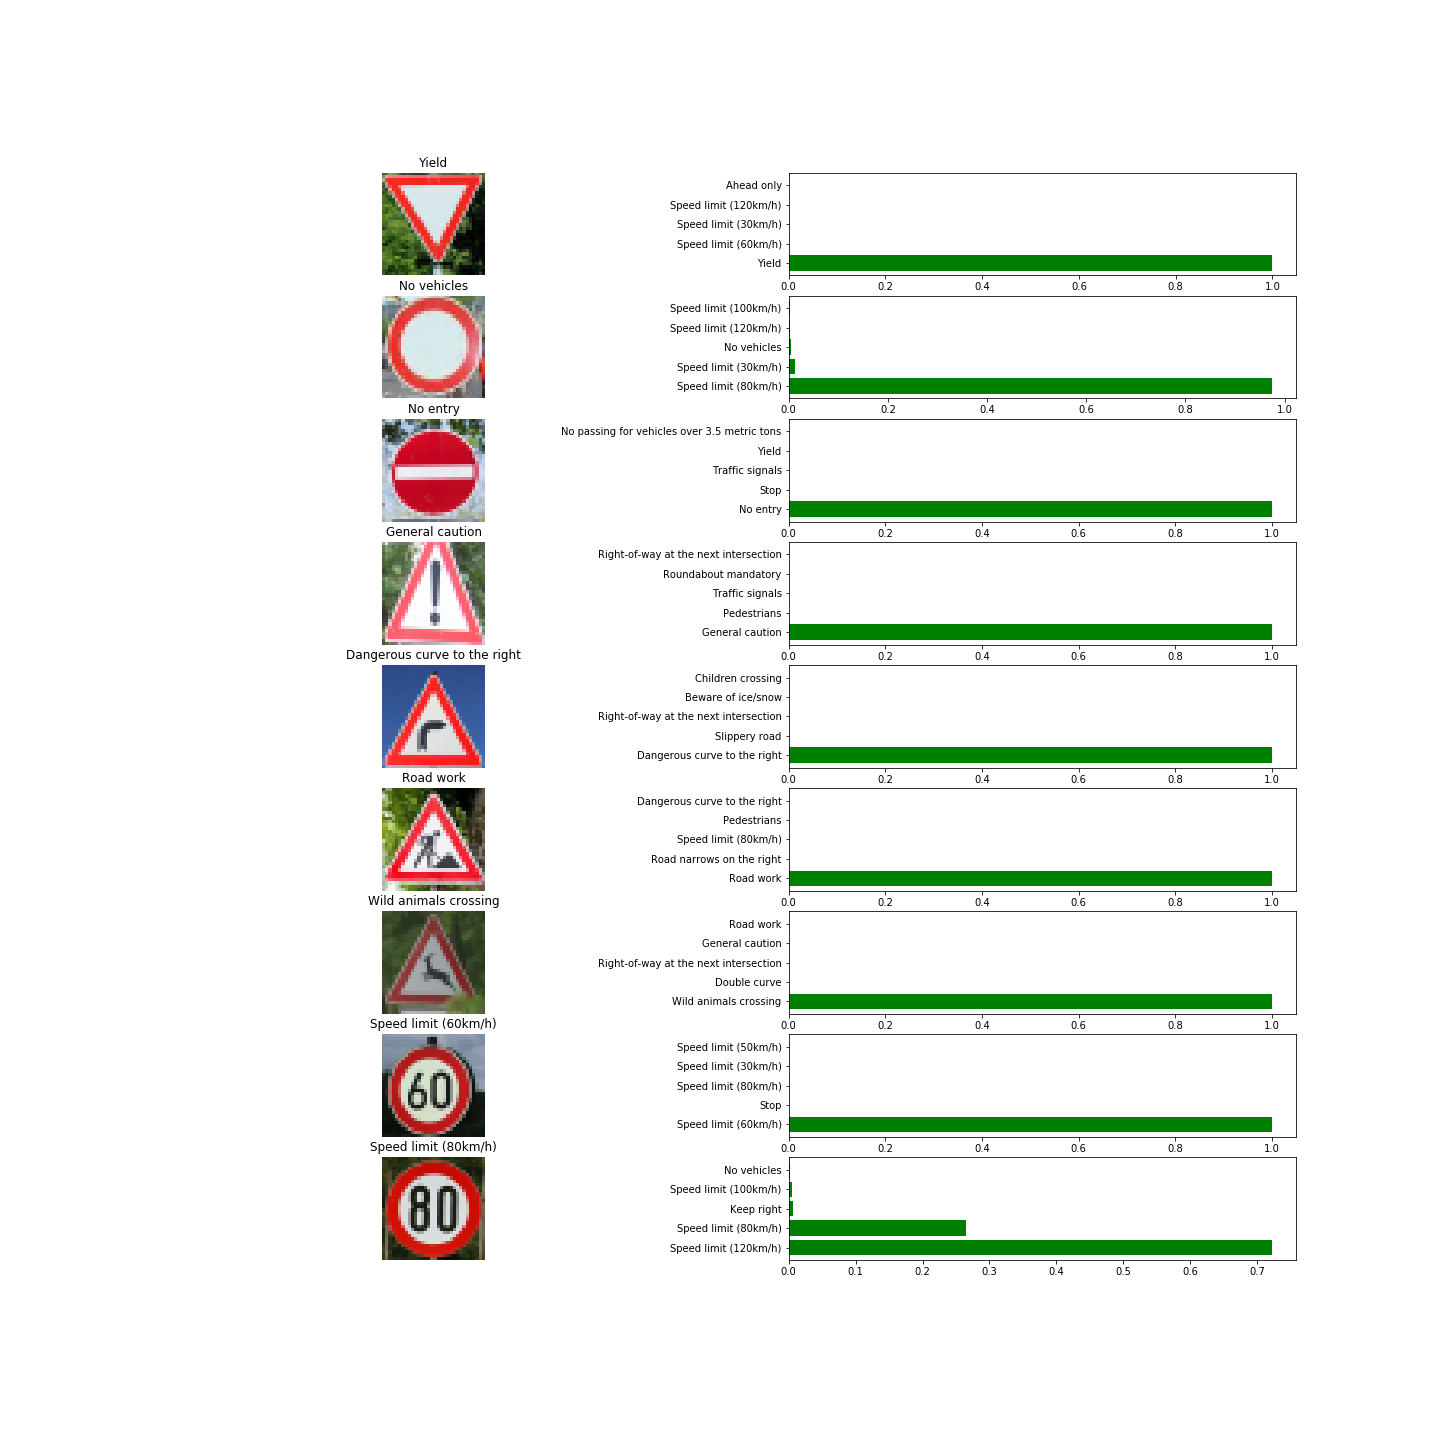
\includegraphics{./images/softmax_prob.png}
\caption{alt text}
\end{figure}

The final trained network was very confident in its guesses for the
correctly recognised 7 images.

The four triangular shaped signs were predicted correctly with the top
probabilities reaching 100\%, however it worth to notice that the
remaining four probabilities are mostly also for triangular shaped
signs. This shape shared by these signs was recognised by the network
very well.

The predictions for the speed limit 60km/h and 80 km/h and no vehicles
signs contain also different speed limit signs, what suggested that
network have no trouble in recognition of unique features of these
signs; a white circle with a red border. Very likely because of this the
no vehicles sign was misclassified as a speed limit 80km/h. A similar
case is for the speed limit 80km/h sign, which was recognised as the
speed limit 120km/h. However, one would expect a misclassification as
different double digits speed limit rather than three digits. It is
worth to highlight that prior this final run the network had not trouble
to recognise all the signs correctly with almost 100\% confidence. As
the all hyperparameters were fixed the reason for this difference is
very likely due to randomness of the generated additional images.

There is still a room for the improvement as demonstrated in
\href{http://yann.lecun.com/exdb/publis/pdf/sermanet-ijcnn-11.pdf}{Traffic
Sign Recognition with Multi-Scale Convolutional Networks} with a network
capable achieving 99.17\% test accuracy for this dataset. But even with
such high accuracy it would interesting exercise to apply these models
to videos, especially from city centres with many ads and other
obstructions, which would make the traffic sign recognition much more
challenging.

See code in Step 3: Softmax Probabilities For Each Image Found on the
Web(\textbf{Traffic\_Sign\_ClassifierFinal.ipynb}).

\hypertarget{optional-visualizing-the-neural-network-see-step-4-of-the-ipython-notebook-for-more-details}{%
\subsubsection{(Optional) Visualizing the Neural Network (See Step 4 of
the Ipython notebook for more
details)}\label{optional-visualizing-the-neural-network-see-step-4-of-the-ipython-notebook-for-more-details}}

\hypertarget{discuss-the-visual-output-of-your-trained-networks-feature-maps.-what-characteristics-did-the-neural-network-use-to-make-classifications}{%
\paragraph{1. Discuss the visual output of your trained network's
feature maps. What characteristics did the neural network use to make
classifications?}\label{discuss-the-visual-output-of-your-trained-networks-feature-maps.-what-characteristics-did-the-neural-network-use-to-make-classifications}}


    % Add a bibliography block to the postdoc
    
    
    
    \end{document}
